
\label{sec:vjetresults}
%\clearpage

In the following, we show the unfolded data distributions for the different jet algorithms under study, comapared to the unfolded MC expectations from Madgraph and Herwig++. The jet mass distributions are studied in 4 leading jet $p_\rm{T}^j$ bins: $125<$ p$_\rm{T}^j$ $<150$ GeV, $150<$ p$_\rm{T}^j$ $<220$ GeV, $220<$ p$_\rm{T}^j$ $<300$ GeV, and $300<$ p$_\rm{T}^j$ $<450$ GeV. For the $R=1.2$ Cambridge Aachen jets, we only study the $\pt$ range above 150 GeV, due to the large radius and the relation $\Delta R \approx 2m/\pt$~\cite{boostedHiggs}. 

In all case, the distributions are truncated in the tails for
visibility purposes. Jet-mass bins with a relative uncertainty larger
than 100\% are not displayed to avoid overlapping with other
$\pt$ bins with a more precise measurement in that bin. 

%We report normalized cross-sections, i.e. $1/\sigma*(d\sigma/dM_J)$ in order to cancel luminosity dependence.
We present normalized cross-sections, as defined in Eq.~\ref{eq:pdf_mjet_simple}.
Both Madgraph and Herwig++ are found to reproduce the data reasonably well: the agreement improves for large $\pt$, while some residual poor modeling is present at low mass, consistent with the dijet analysis results. % (that is also the most sensitive region to PU effects). %It is also interesting to observe that the more aggressive the grooming is, the more herwig seems to better reproduce the data than madgraph/pythia. 


\subsection{Z$(\ell\ell)$+ jet Analysis}

Fig.~\ref{figs:AK7ZmmInt1}-\ref{figs:AK7ZmmInt4} show the jet mass distribution for AK7 jets in Z$(\ell\ell)$ +jet events for the different clustering algorithm studied: ungroomed, pruned, trimmed and filtered respectively.  

\begin{figure}[!htb]
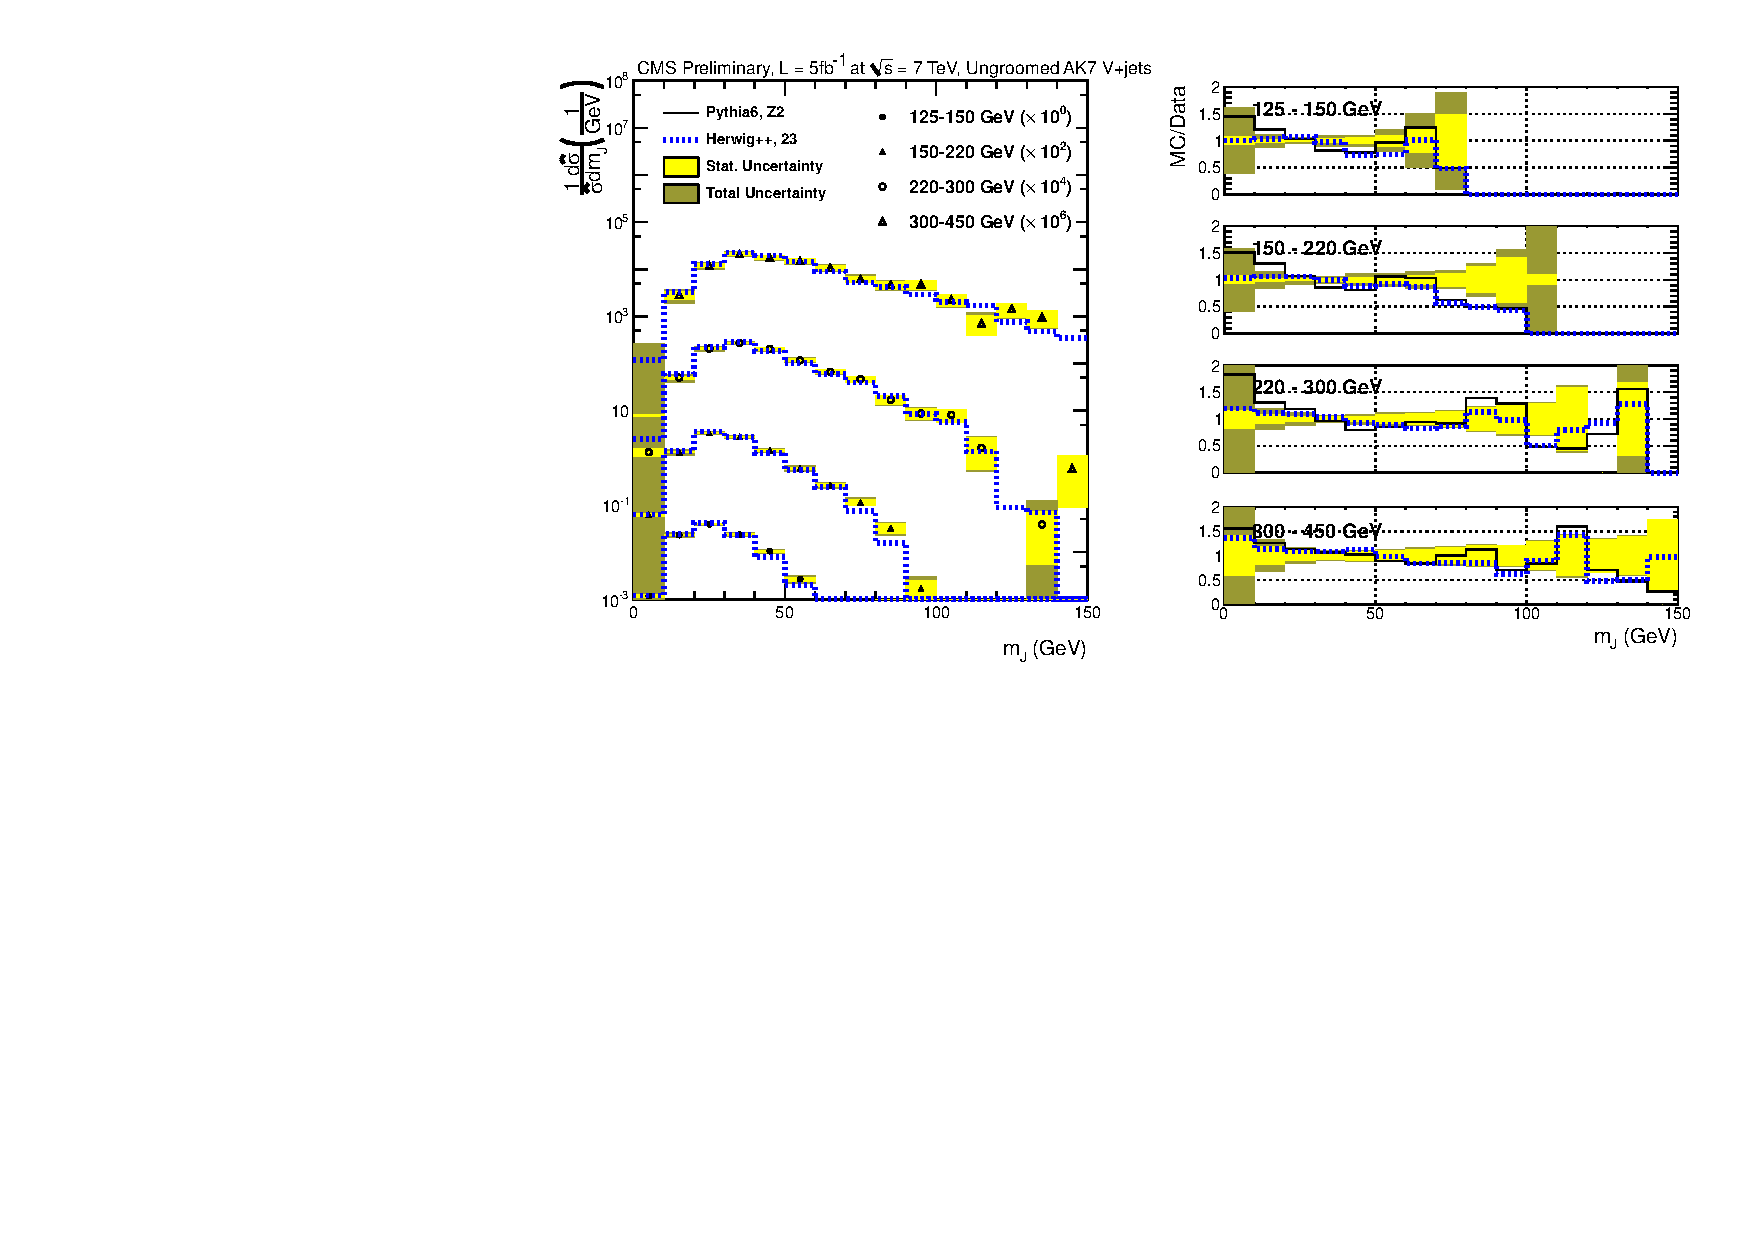
\includegraphics[width=0.99\textwidth]{figs/Zll/jetmassunf_ak7_log.pdf}
\caption{Unfolded AK7 ungroomed jet mass distribution for Z$(\ell\ell)$+ jet events. The data (black points) are compared to the MC expectations from Madgraph (solid red) and herwigpp (solid blue).}
\label{figs:AK7ZmmInt1}
\end{figure}

\begin{figure}[!htb]
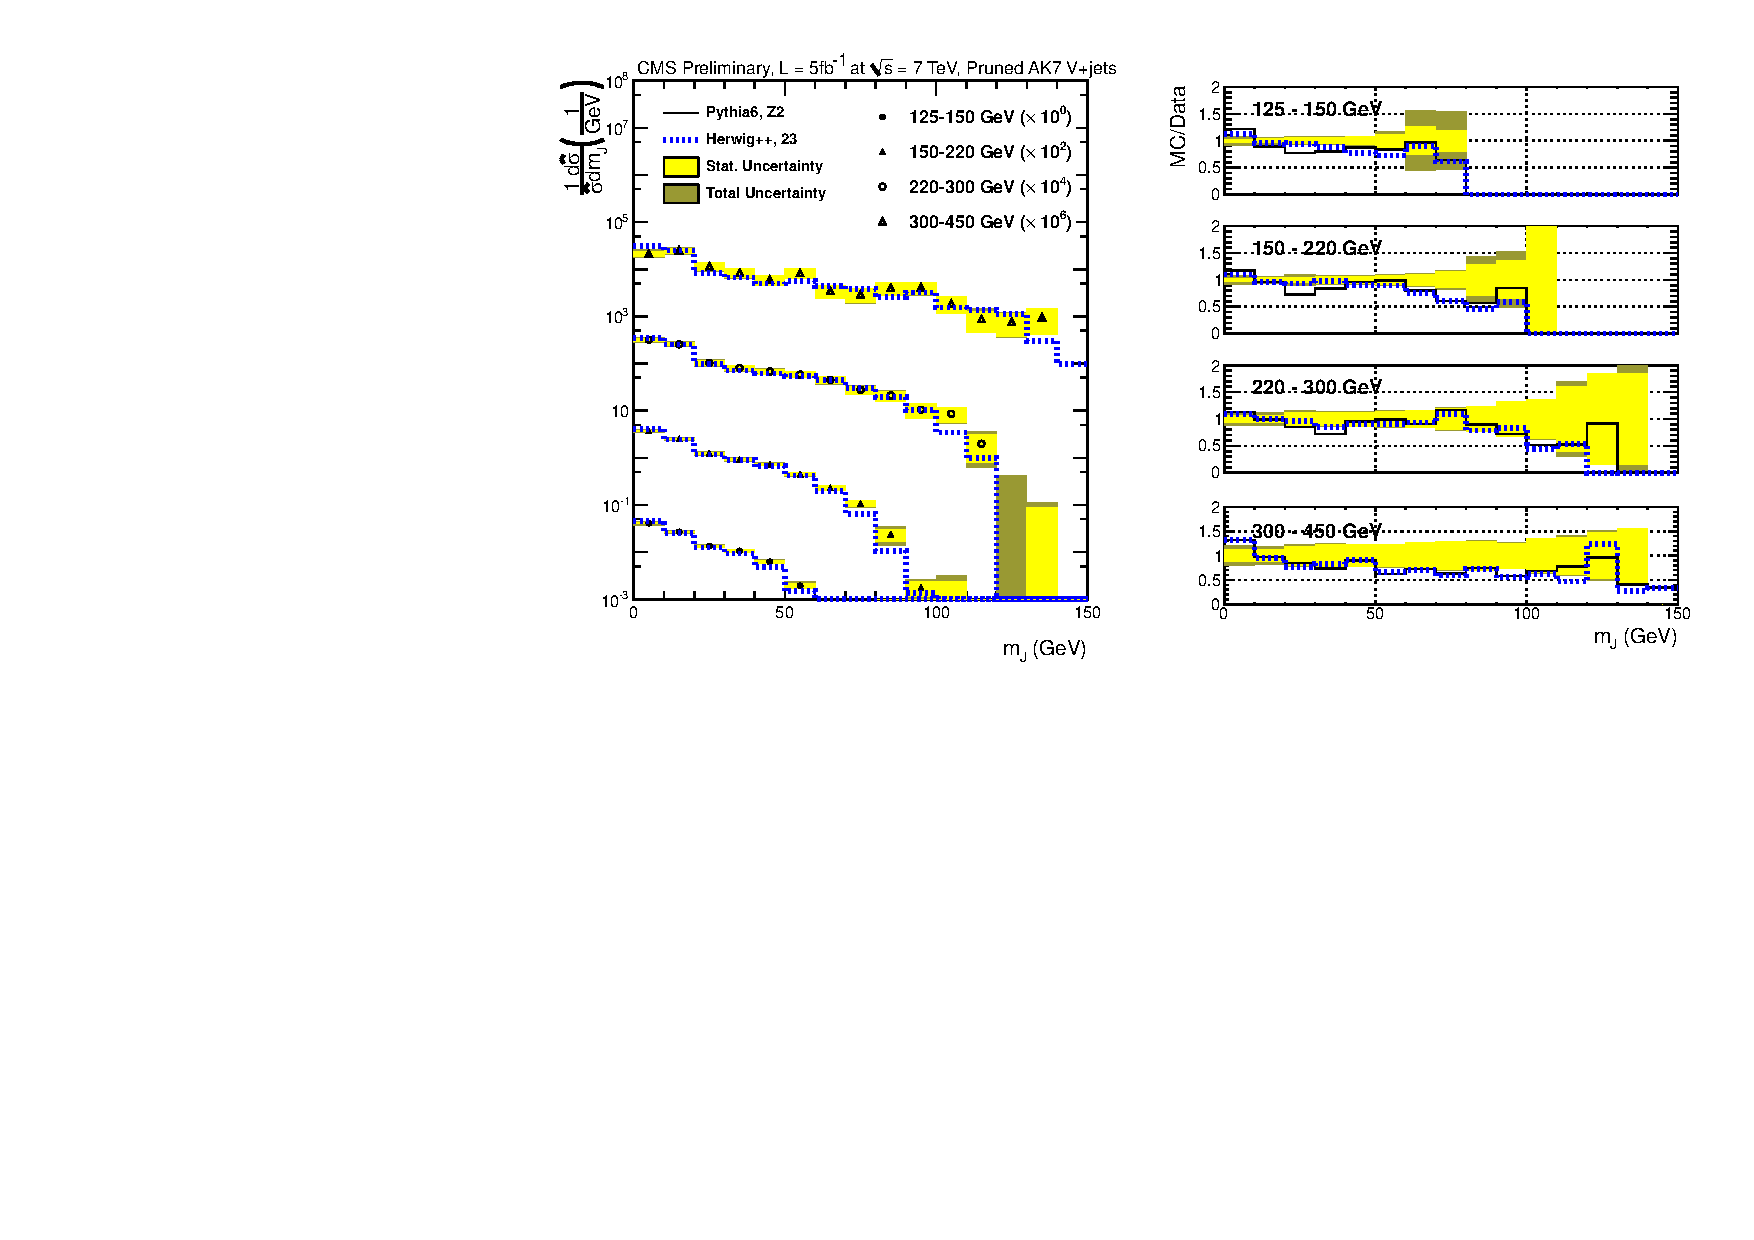
\includegraphics[width=0.99\textwidth]{figs/Zll/jetmassunf_ak7pr_log.pdf}
\caption{Unfolded AK7 pruned jet mass distribution for Z$(\ell\ell)$+ jet events. The data (black points) are compared to the MC expectations from Madgraph (solid red) and herwigpp (solid blue).}
\label{figs:AK7ZmmInt2}
\end{figure}

\begin{figure}[!htb]
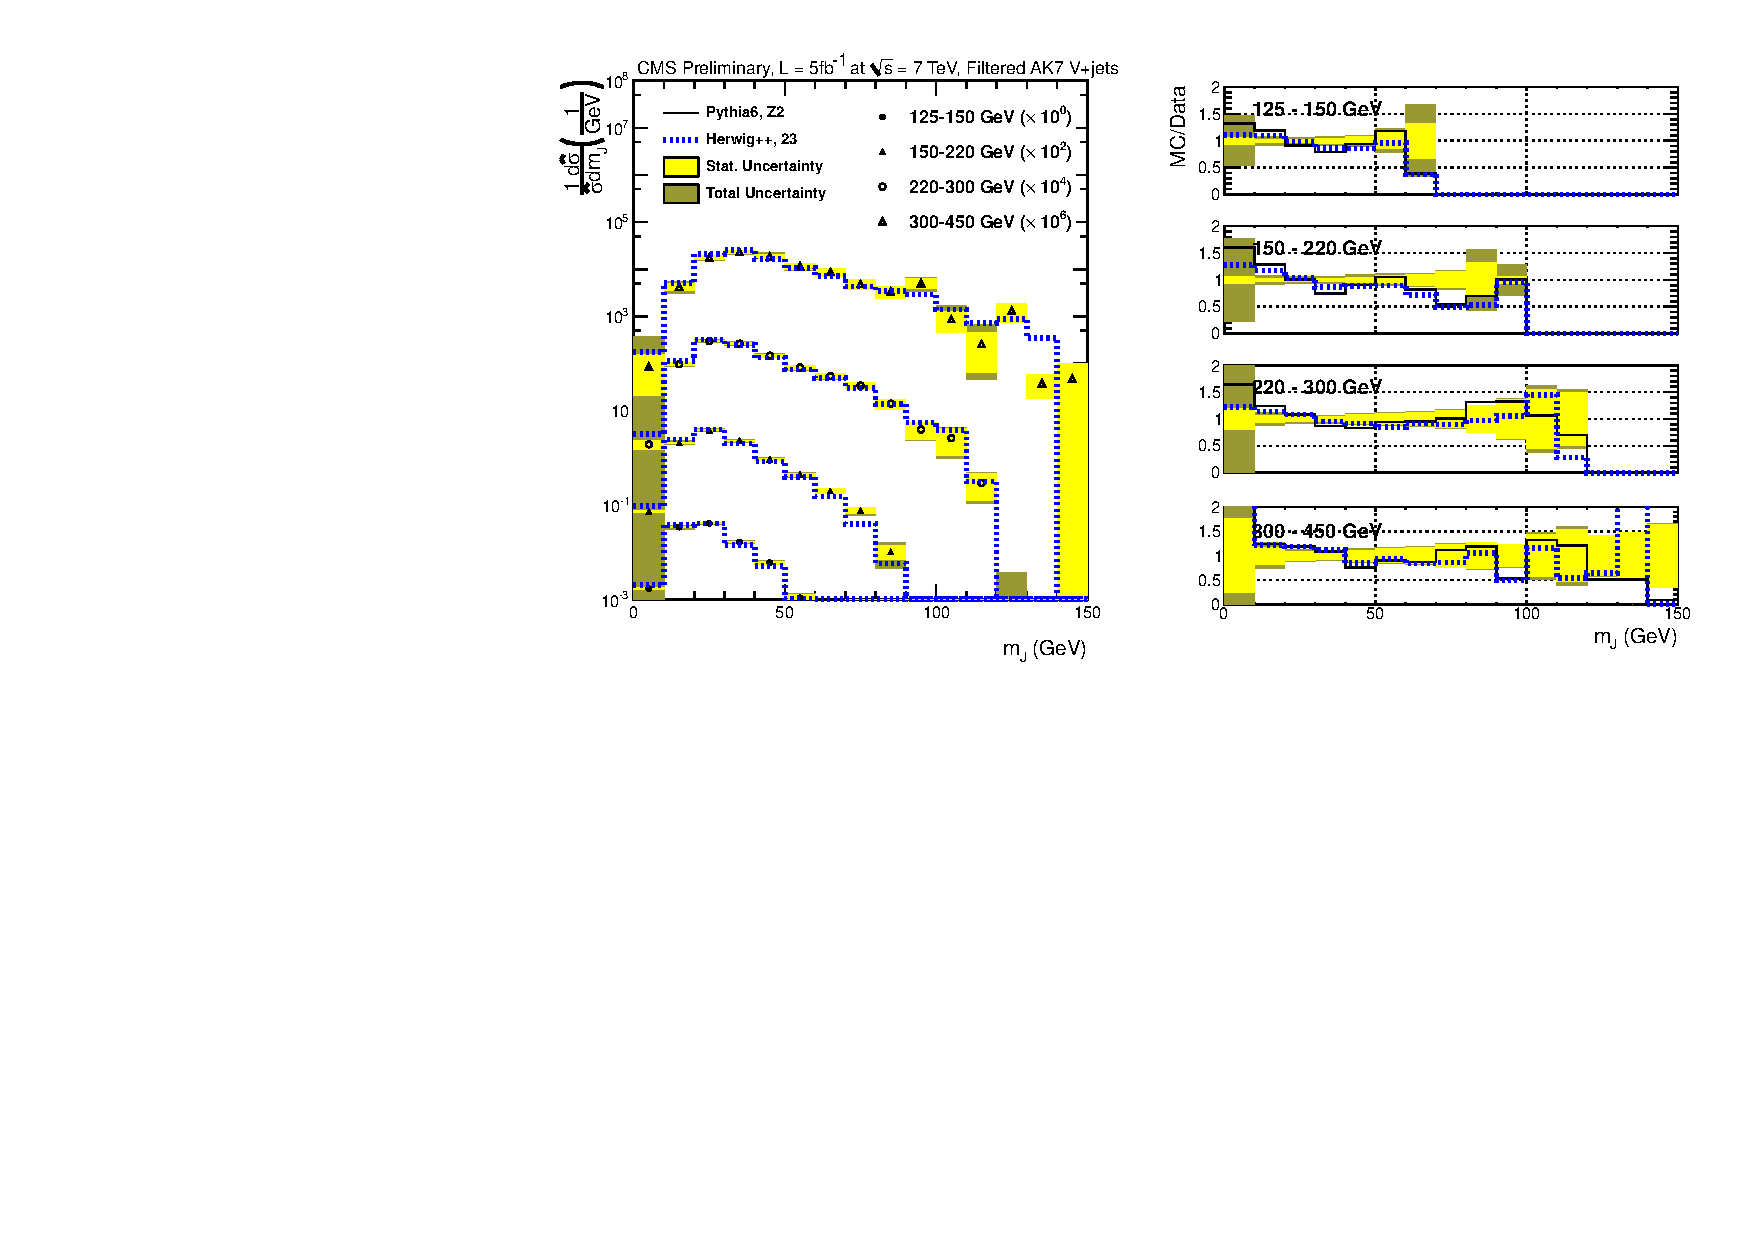
\includegraphics[width=0.99\textwidth]{figs/Zll/jetmassunf_ak7ft_log.pdf}
\caption{Unfolded AK7 filtered jet mass distribution for Z$(\ell\ell)$+ jet events. The data (black points) are compared to the MC expectations from Madgraph (solid red) and herwigpp (solid blue).}
\label{figs:AK7ZmmInt3}
\end{figure}

\begin{figure}[!htb]
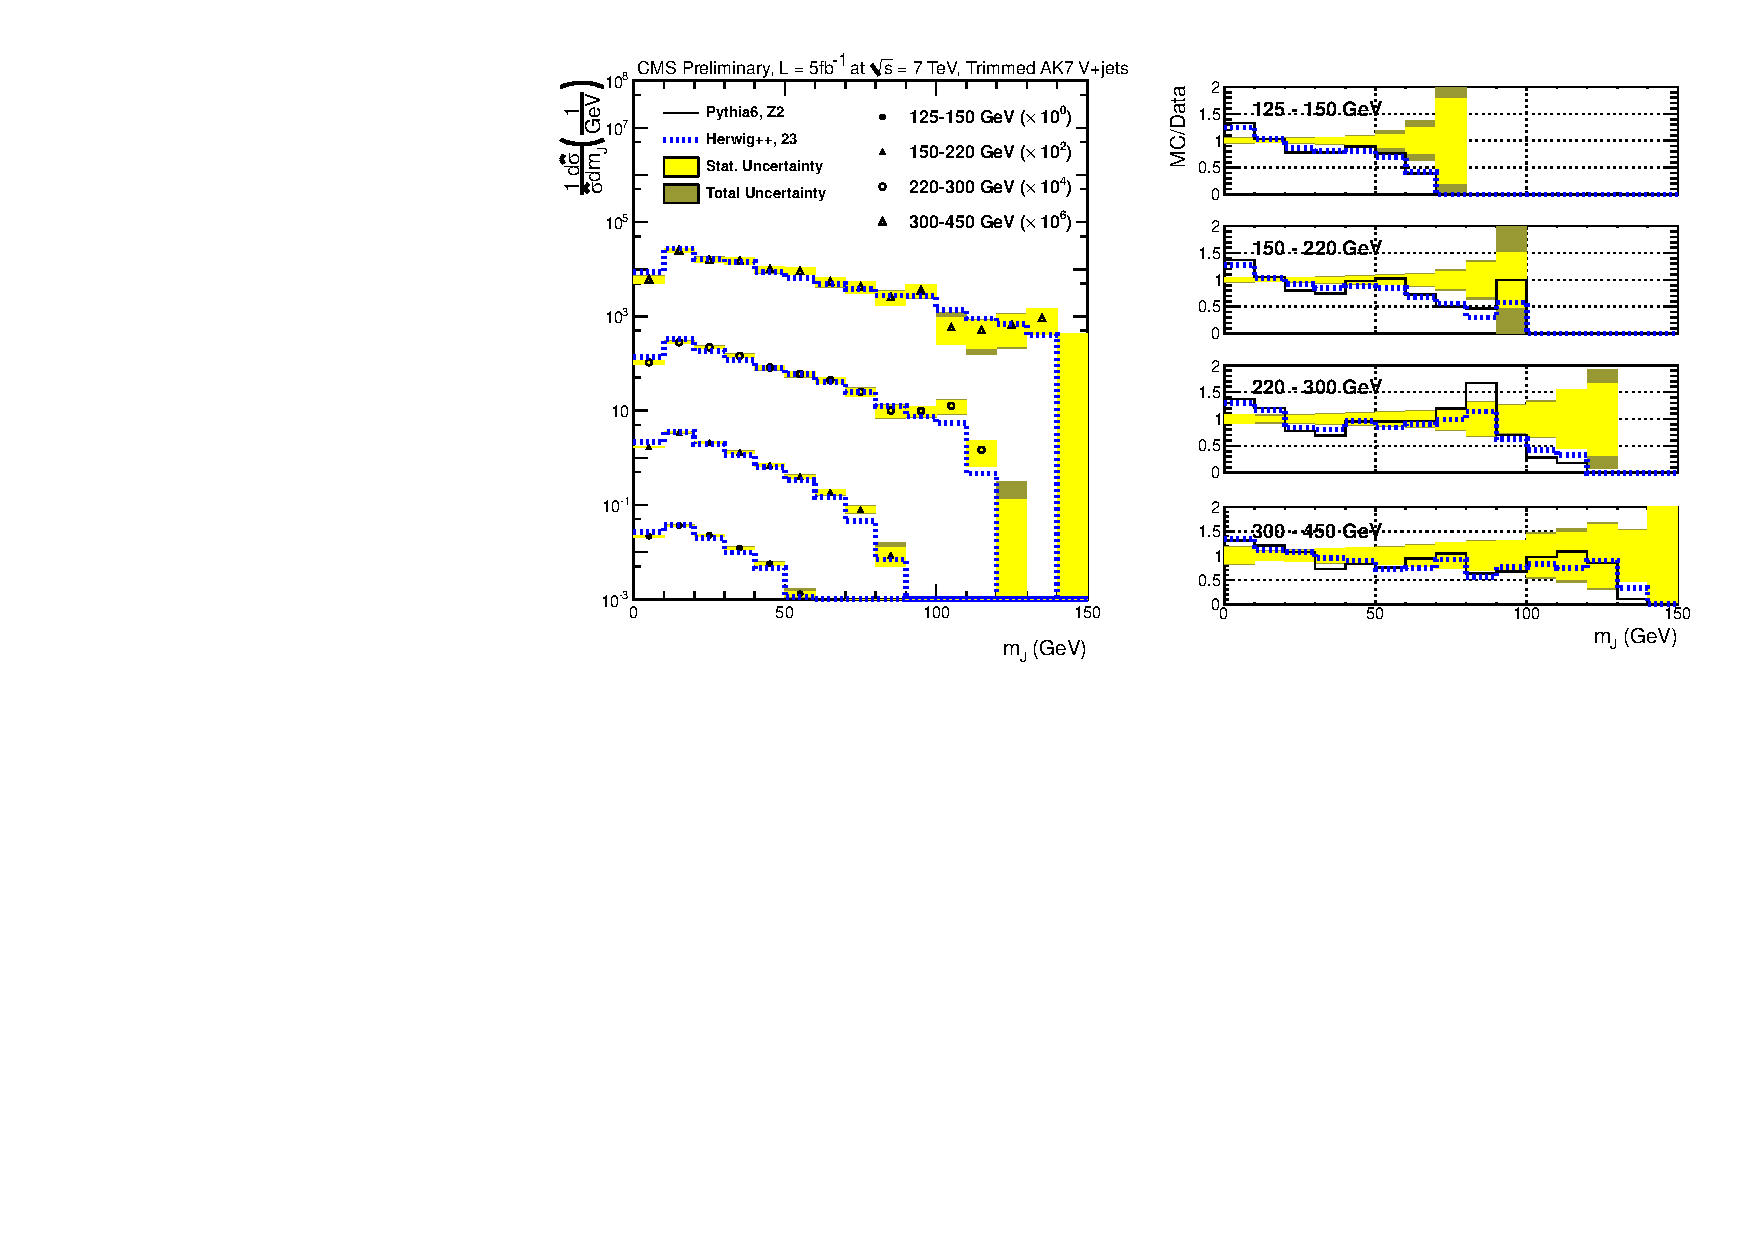
\includegraphics[width=0.99\textwidth]{figs/Zll/jetmassunf_ak7tr_log.pdf}
\caption{Unfolded AK7 trimmed jet mass distribution for Z$(\ell\ell)$+ jet events. The data (black points) are compared to the MC expectations from Madgraph (solid red) and herwigpp (solid blue).}
\label{figs:AK7ZmmInt4}
\end{figure}


Fig.~\ref{figs:prunedZmmInt1}-\ref{figs:prunedZmmInt2} show the jet mass distribution for pruned CA 0.8 and filtered CA 1.2 jets in Z$(\ell\ell)$ +jet events.
 
\begin{figure}[!htb]
\centering
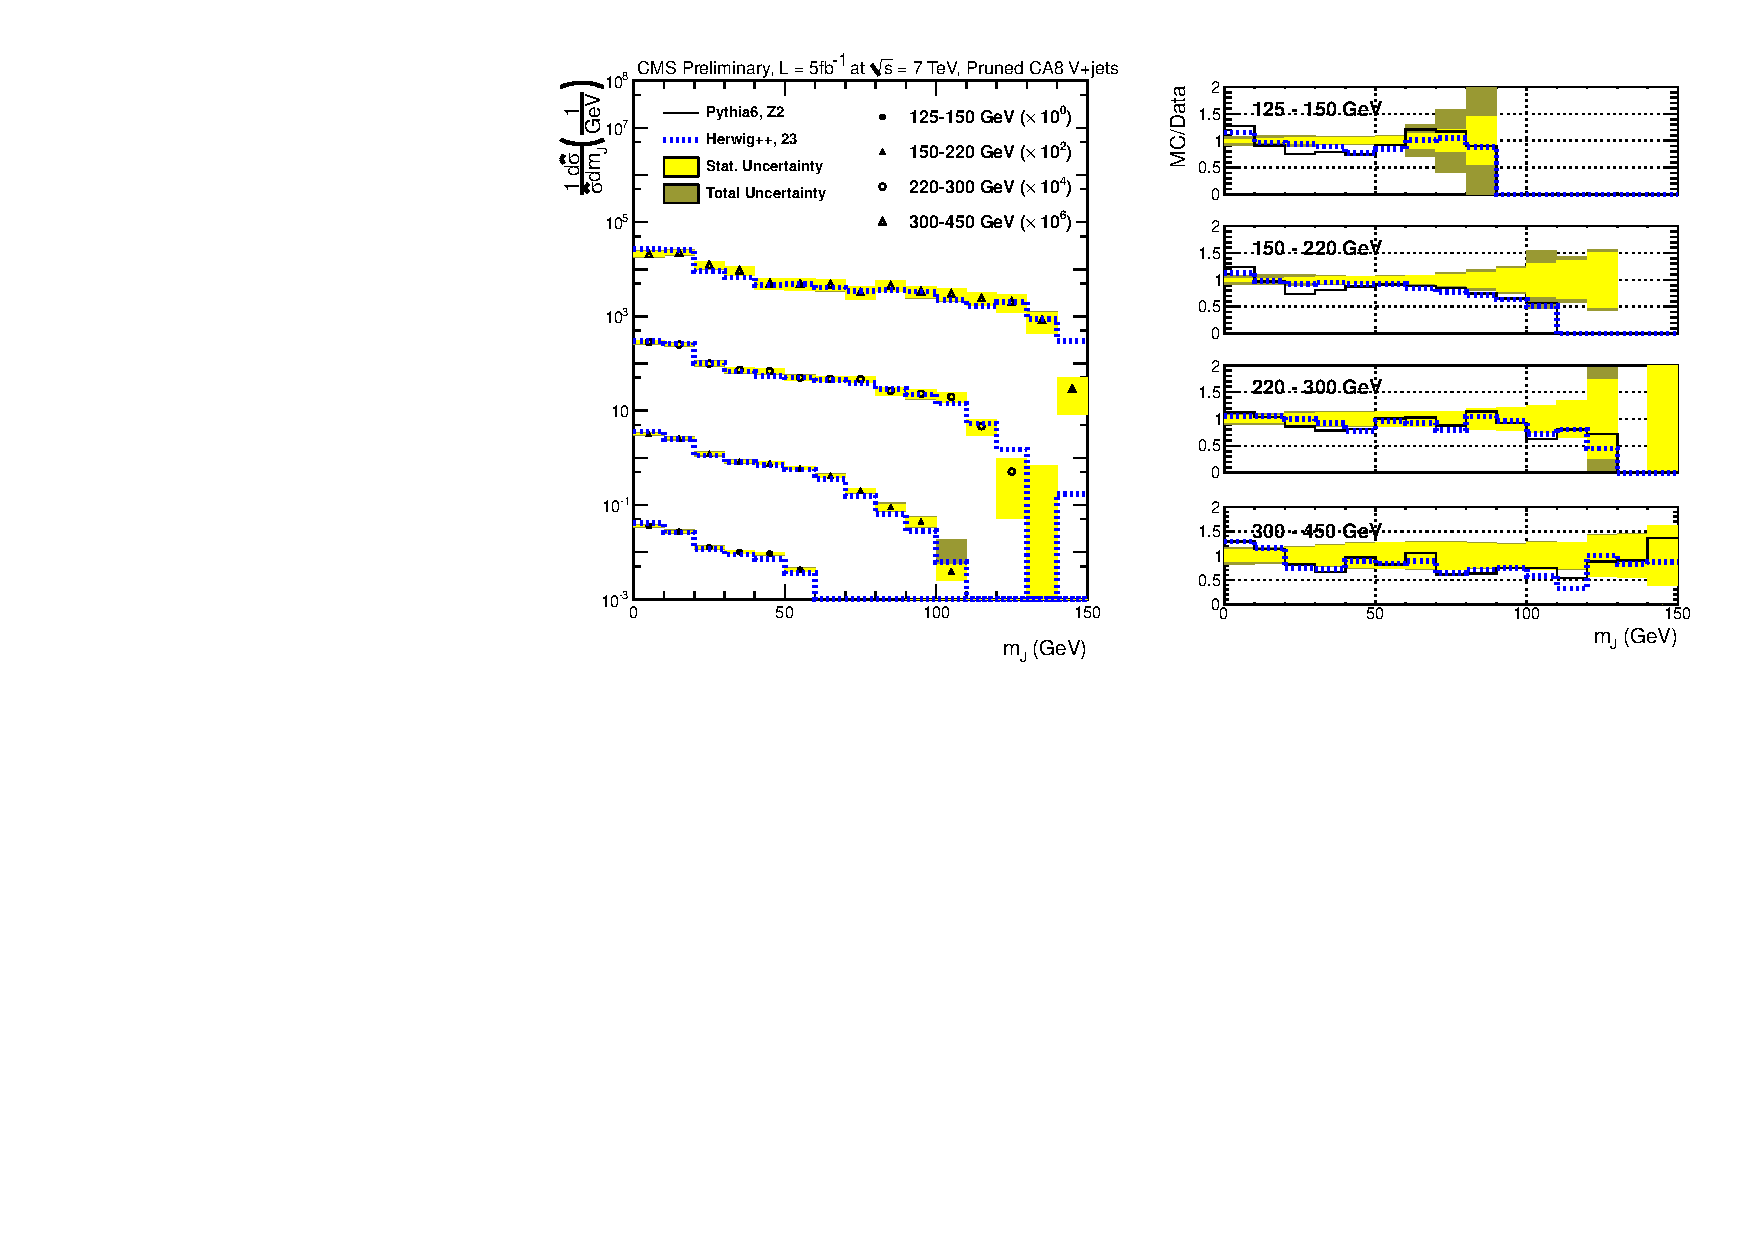
\includegraphics[width=0.99\textwidth]{figs/Zll/jetmassunf_ca8pr_log.pdf}
\caption{Unfolded CA 0.8 pruned jet mass distribution for Z$(\ell\ell)$+ jet events. The data (black points) are compared to the MC expectations from Madgraph (solid red) and herwigpp (solid blue).}
\label{figs:prunedZmmInt1}
\end{figure}

\begin{figure}[!htb]
\centering
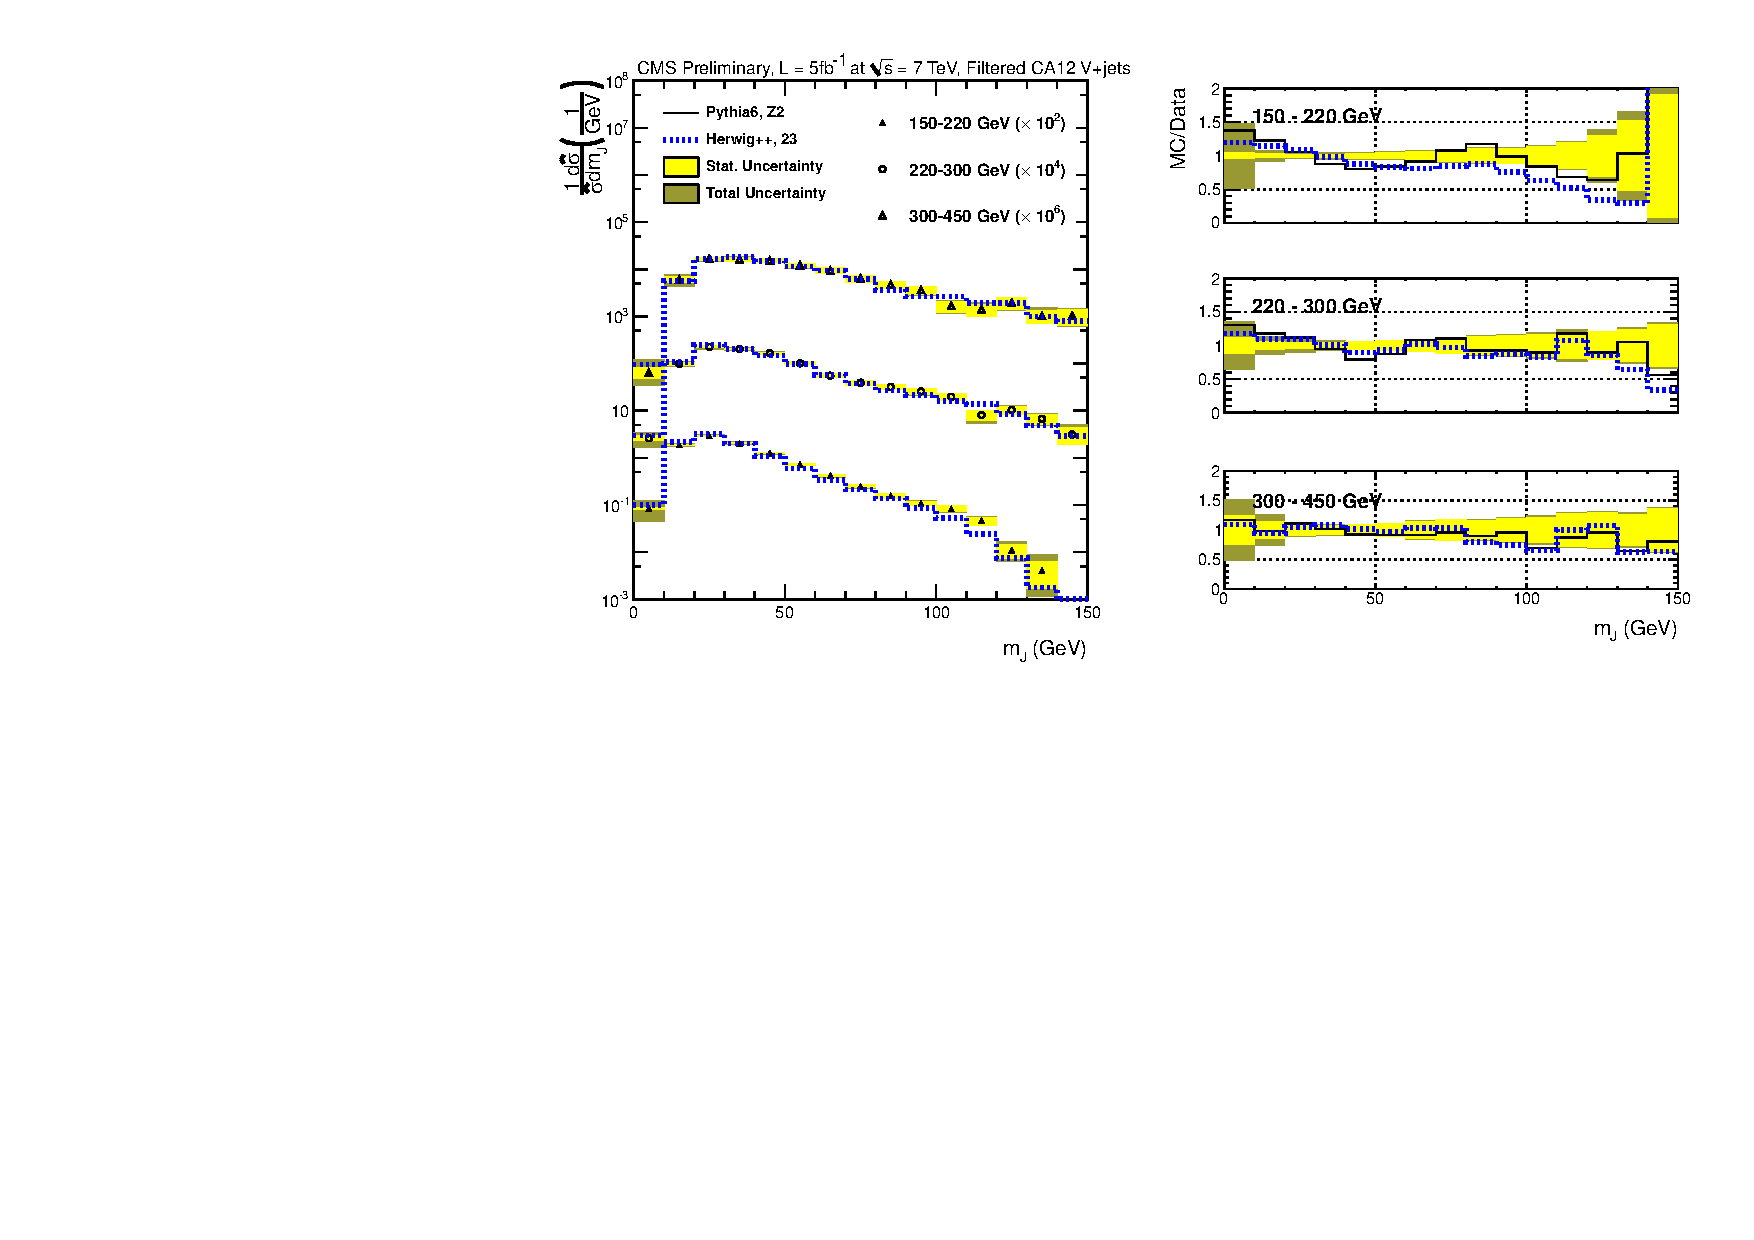
\includegraphics[width=0.99\textwidth]{figs/Zll/jetmassunf_ca12ft_log.pdf}
\caption{Unfolded CA 1.2 filtered jet mass distribution for Z$(\ell\ell)$+ jet events. The data (black points) are compared to the MC expectations from Madgraph (solid red) and herwigpp (solid blue).}
\label{figs:prunedZmmInt2}
\end{figure}


\clearpage


\subsection{W$(\ell\nu)$ + jet Analysis}

Fig.~\ref{figs:AK7WmnInt1}-\ref{figs:AK7WmnInt4} shows the jet mass distribution for AK7 jets in W$(\ell\nu)$ +jet events, for the different clustering algorithm studied: ungroomed, pruned, trimmed and filtered respectively.

\begin{figure}[!htb]
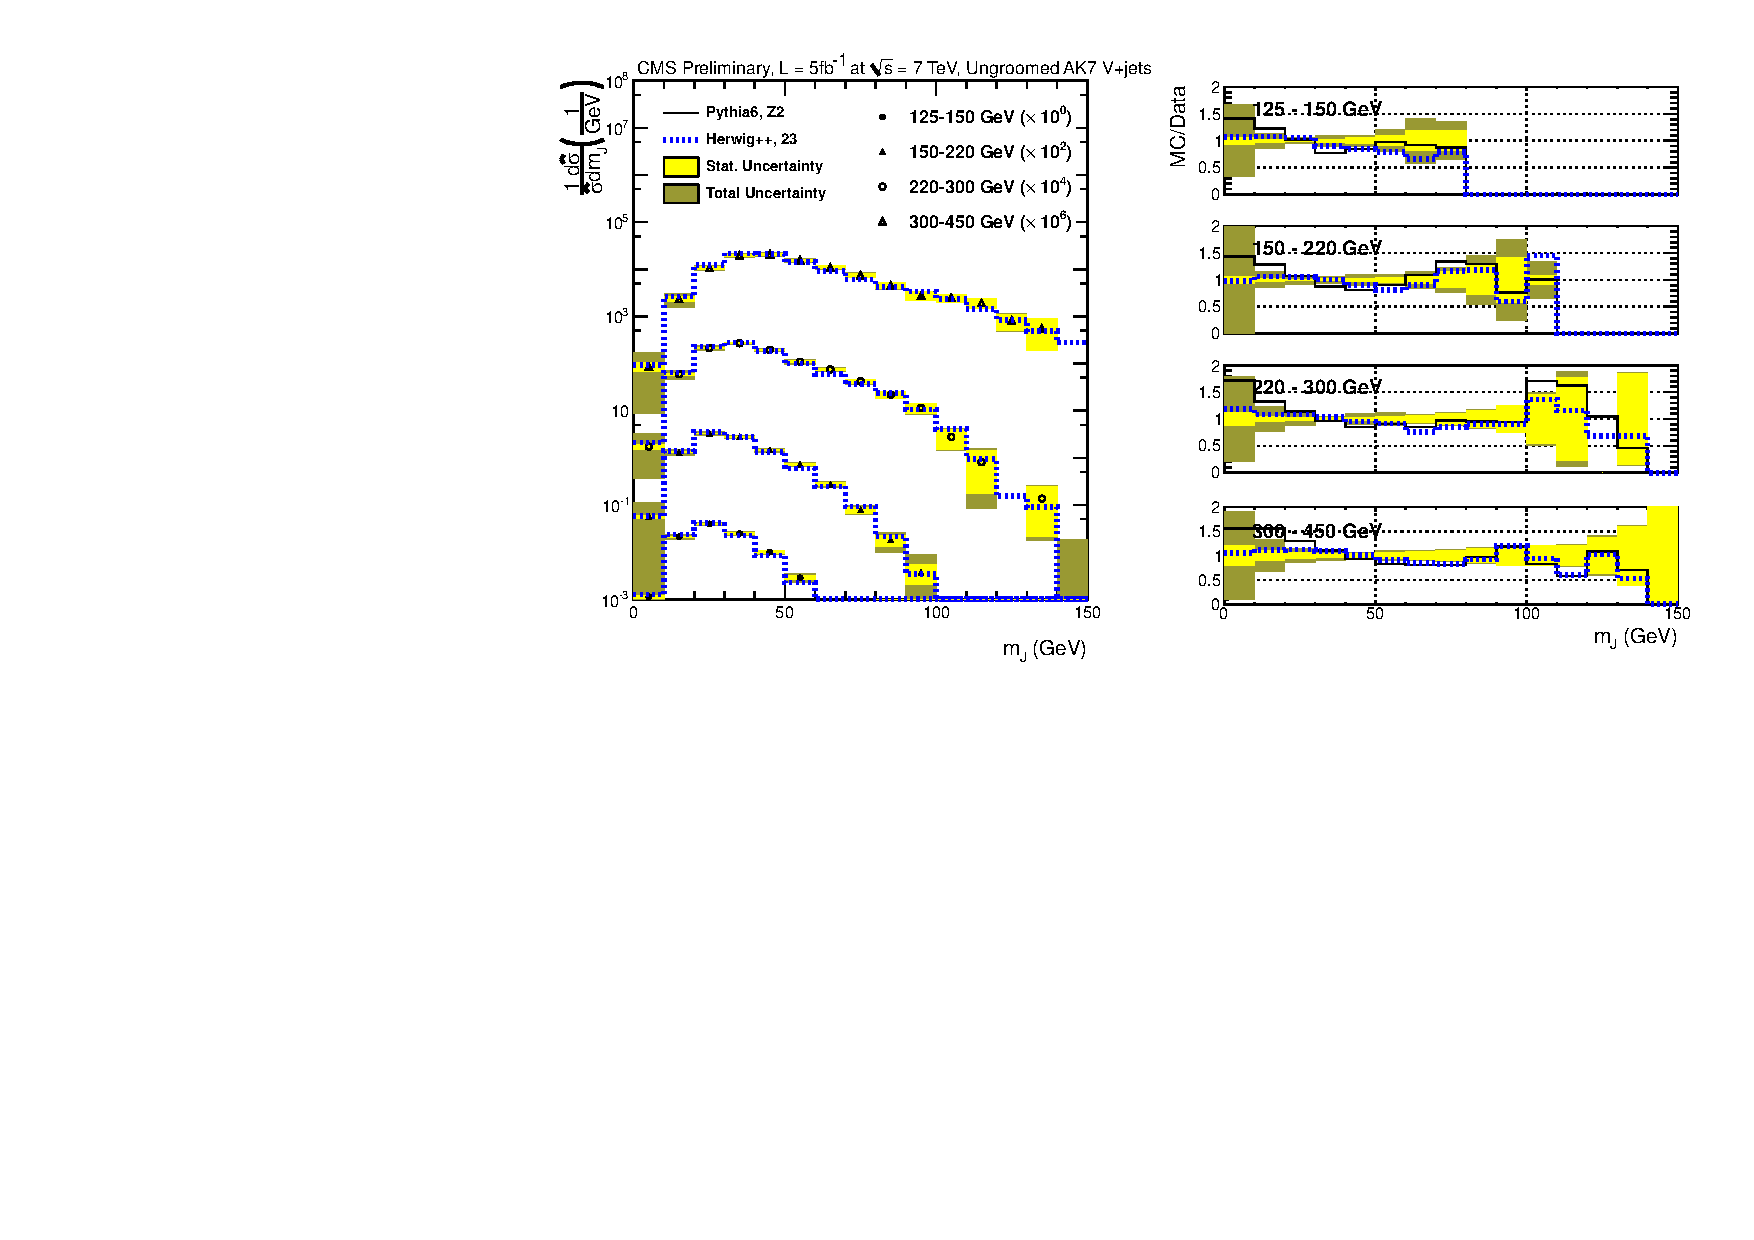
\includegraphics[width=0.99\textwidth]{figs/Wln/jetmassunf_ak7_log.pdf}
\caption{Unfolded AK7 ungroomed jet mass distribution for W$(\ell\nu)$+ jet events. The data (black points) are compared to the MC expectations from Madgraph (solid red) and herwigpp (solid blue).}
\label{figs:AK7WmnInt1}
\end{figure}

\begin{figure}[!htb]
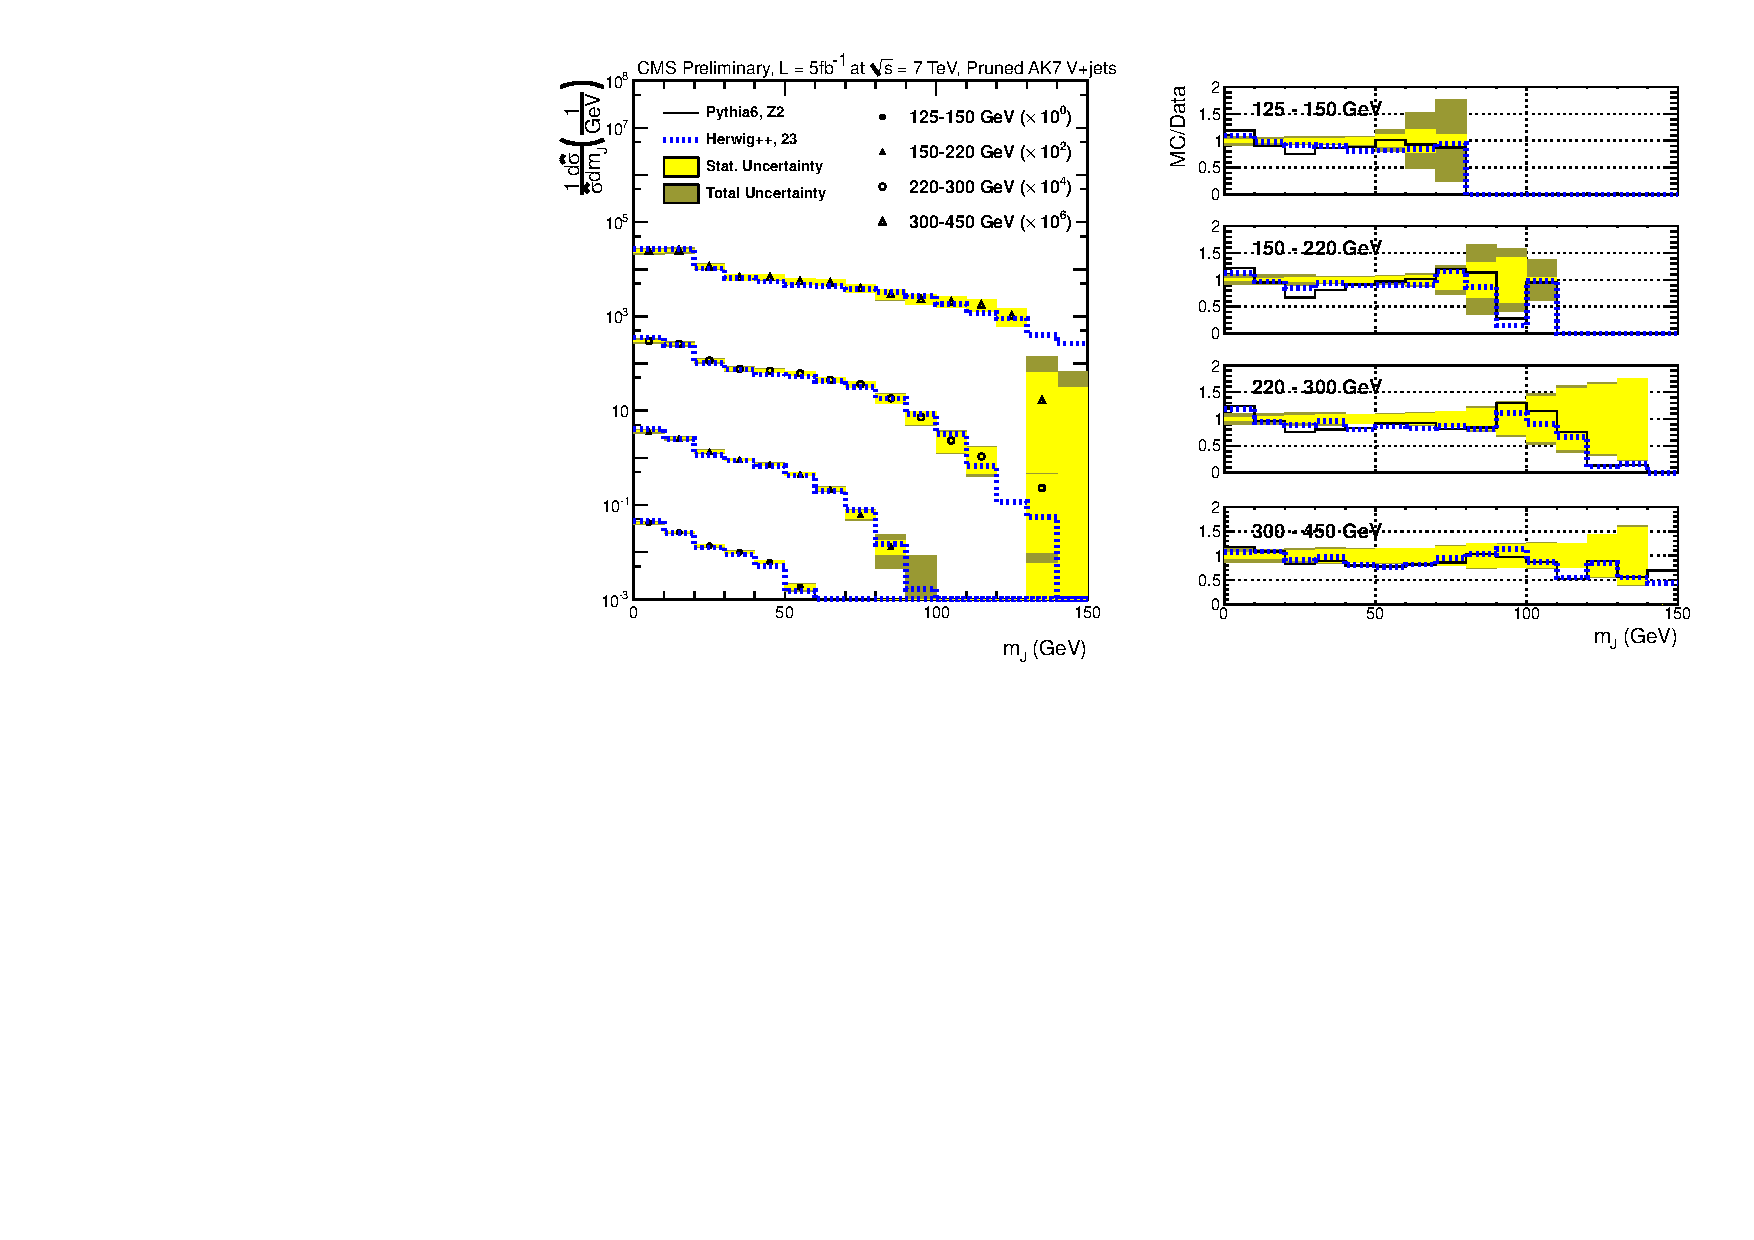
\includegraphics[width=0.99\textwidth]{figs/Wln/jetmassunf_ak7pr_log.pdf}
\caption{Unfolded AK7 pruned jet mass distribution for W$(\ell\nu)$+ jet events. The data (black points) are compared to the MC expectations from Madgraph (solid red) and herwigpp (solid blue).}
\label{figs:AK7WmnInt2}
\end{figure}

\begin{figure}[!htb]
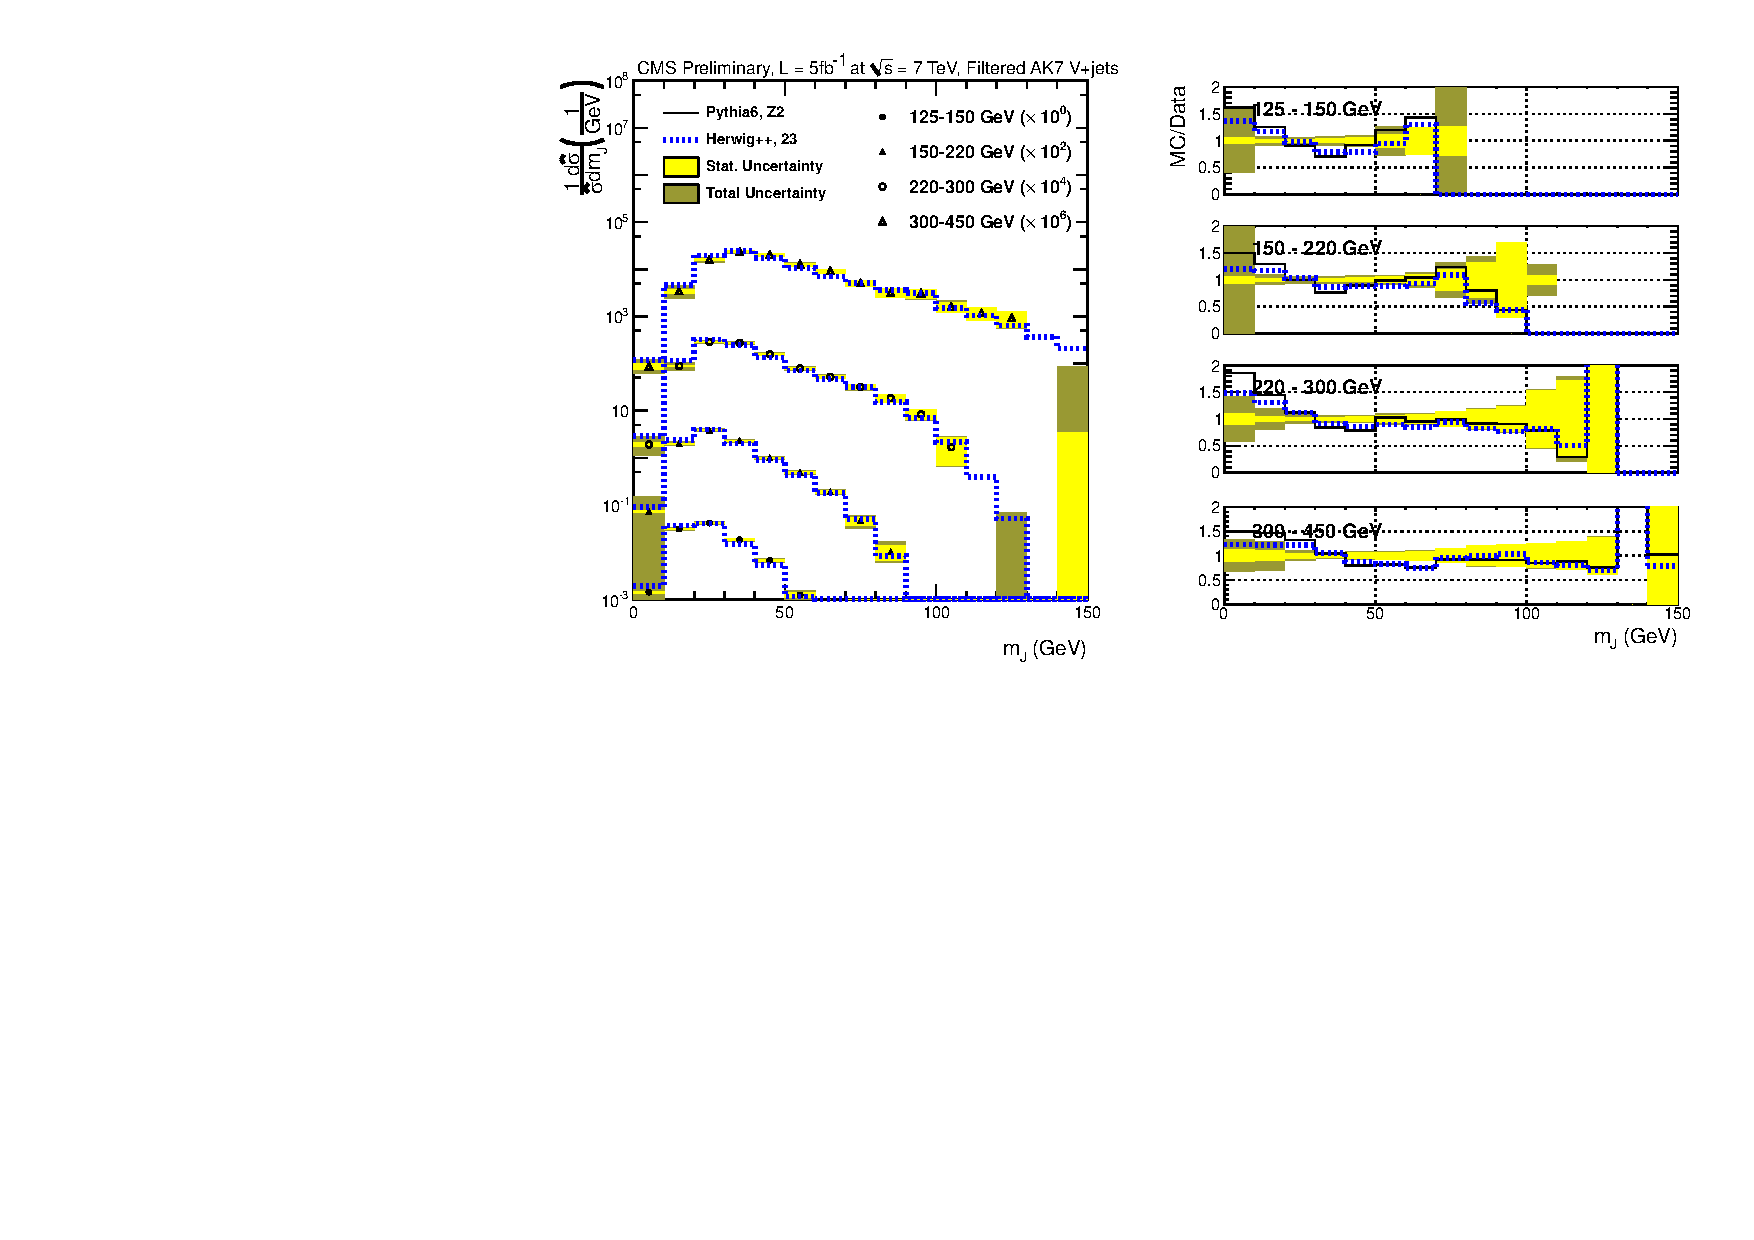
\includegraphics[width=0.99\textwidth]{figs/Wln/jetmassunf_ak7ft_log.pdf}
\caption{Unfolded AK7 filtered jet mass distribution for W$(\ell\nu)$+ jet events. The data (black points) are compared to the MC expectations from Madgraph (solid red) and herwigpp (solid blue).}
\label{figs:AK7WmnInt3}
\end{figure}

\begin{figure}[!htb]
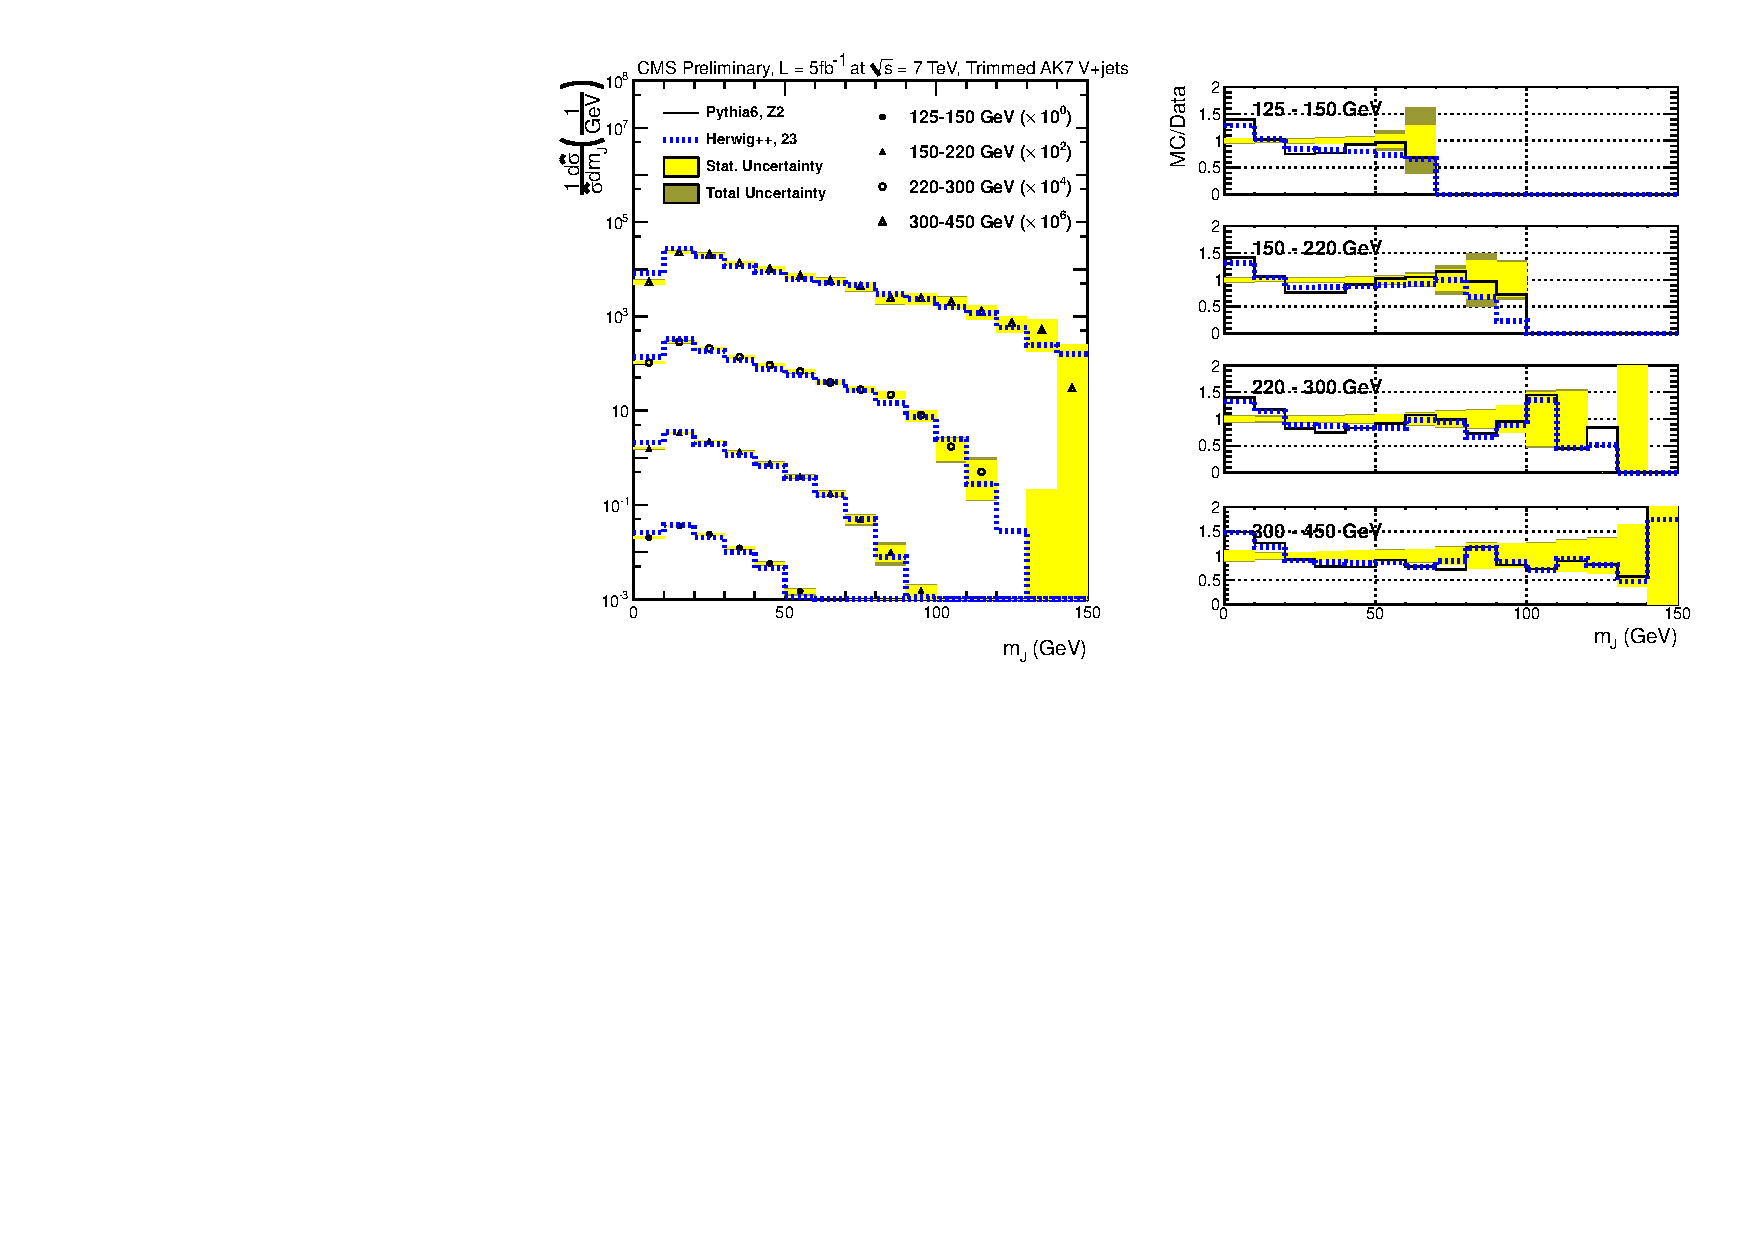
\includegraphics[width=0.99\textwidth]{figs/Wln/jetmassunf_ak7tr_log.pdf}
\caption{Unfolded AK7 trimmed jet mass distribution for W$(\ell\nu)$+ jet events. The data (black points) are compared to the MC expectations from Madgraph (solid red) and herwigpp (solid blue).}
\label{figs:AK7WmnInt4}
\end{figure}



Fig.~\ref{figs:prunedWmnInt1}-\ref{figs:prunedWmnInt2} shows the jet mass distribution for pruned CA 0.8 and filtered CA 1.2 jets in W$(\ell\nu)$ +jet events.

\begin{figure}[!htb]
\centering
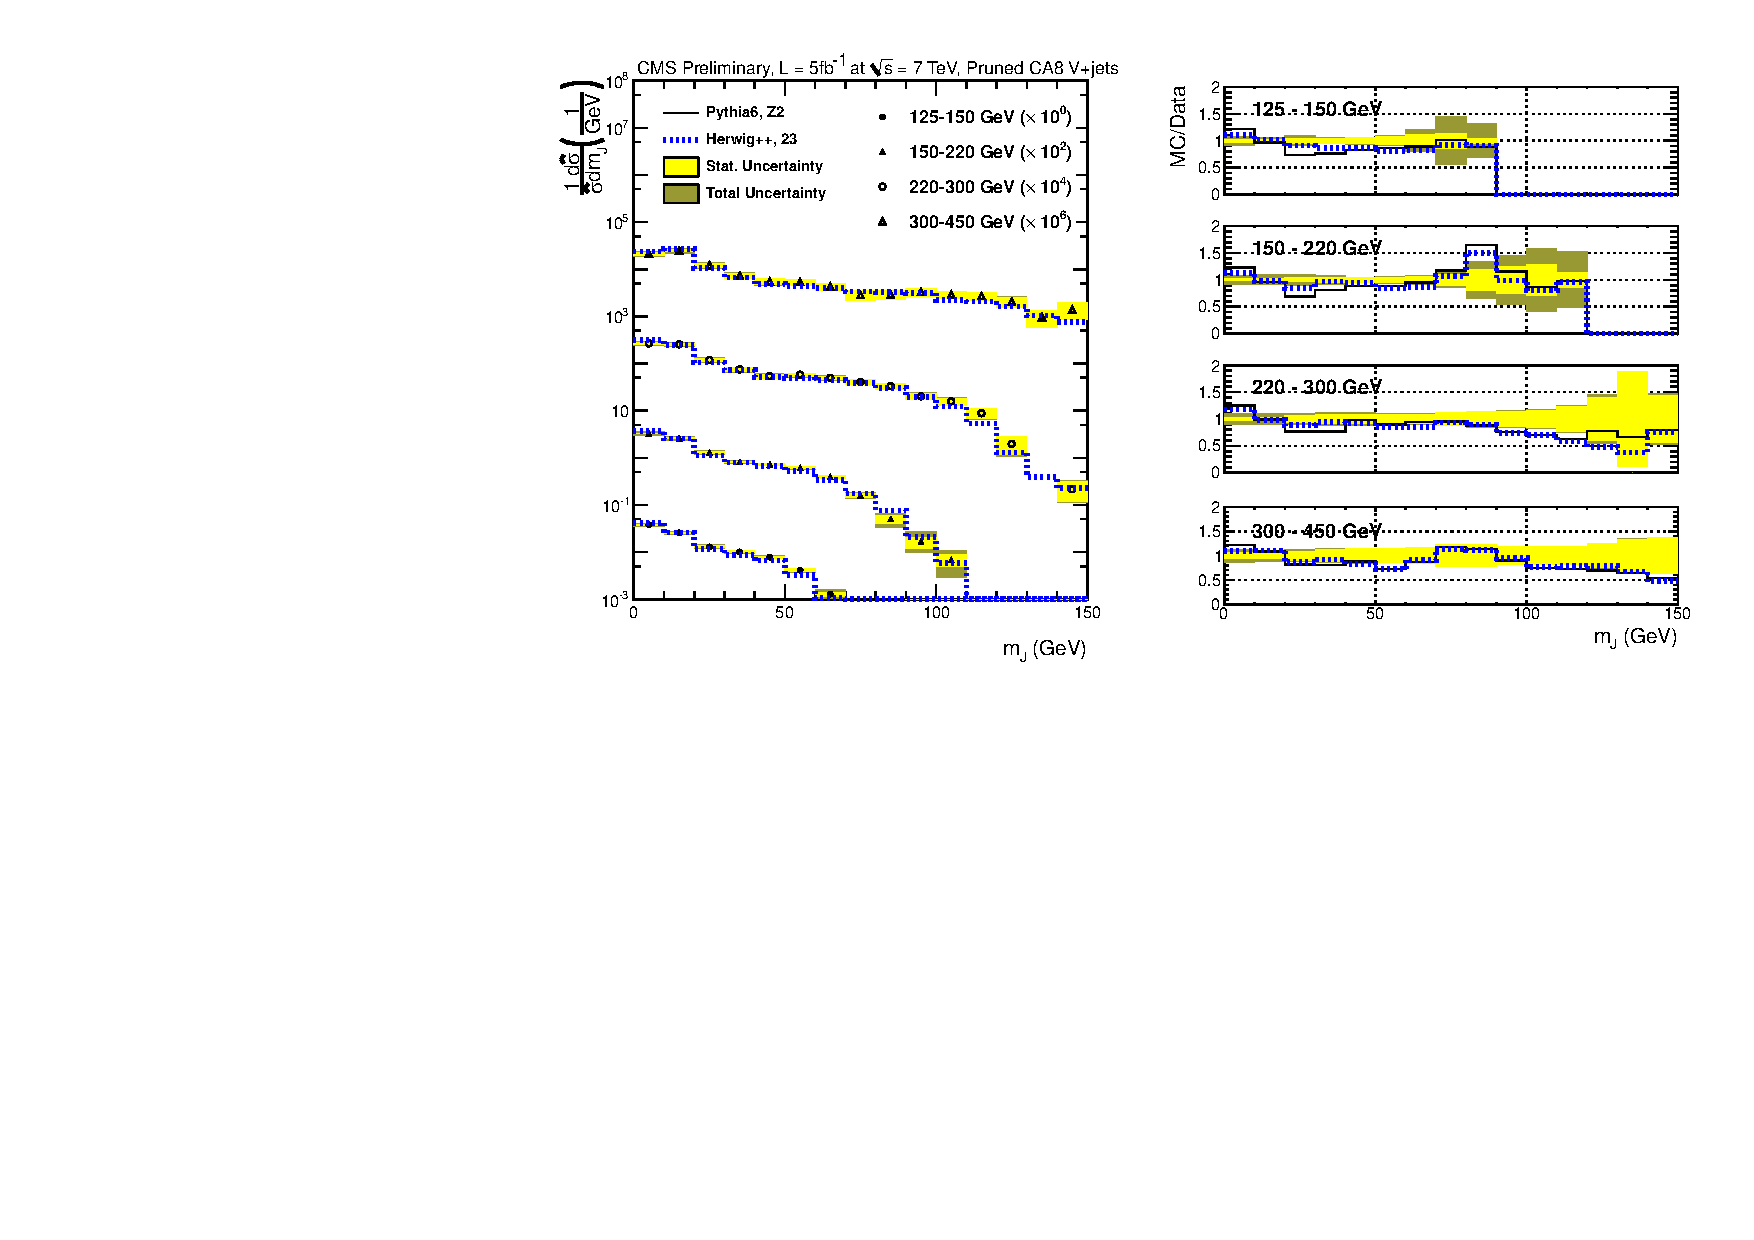
\includegraphics[width=0.99\textwidth]{figs/Wln/jetmassunf_ca8pr_log.pdf}
\caption{Unfolded CA 0.8 pruned jet mass distribution for W$(\ell\nu)$+ jet events. The data (black points) are compared to the MC expectations from Madgraph (solid red) and herwigpp (solid blue).}
\label{figs:prunedWmnInt1}
\end{figure}

\begin{figure}[!htb]
\centering
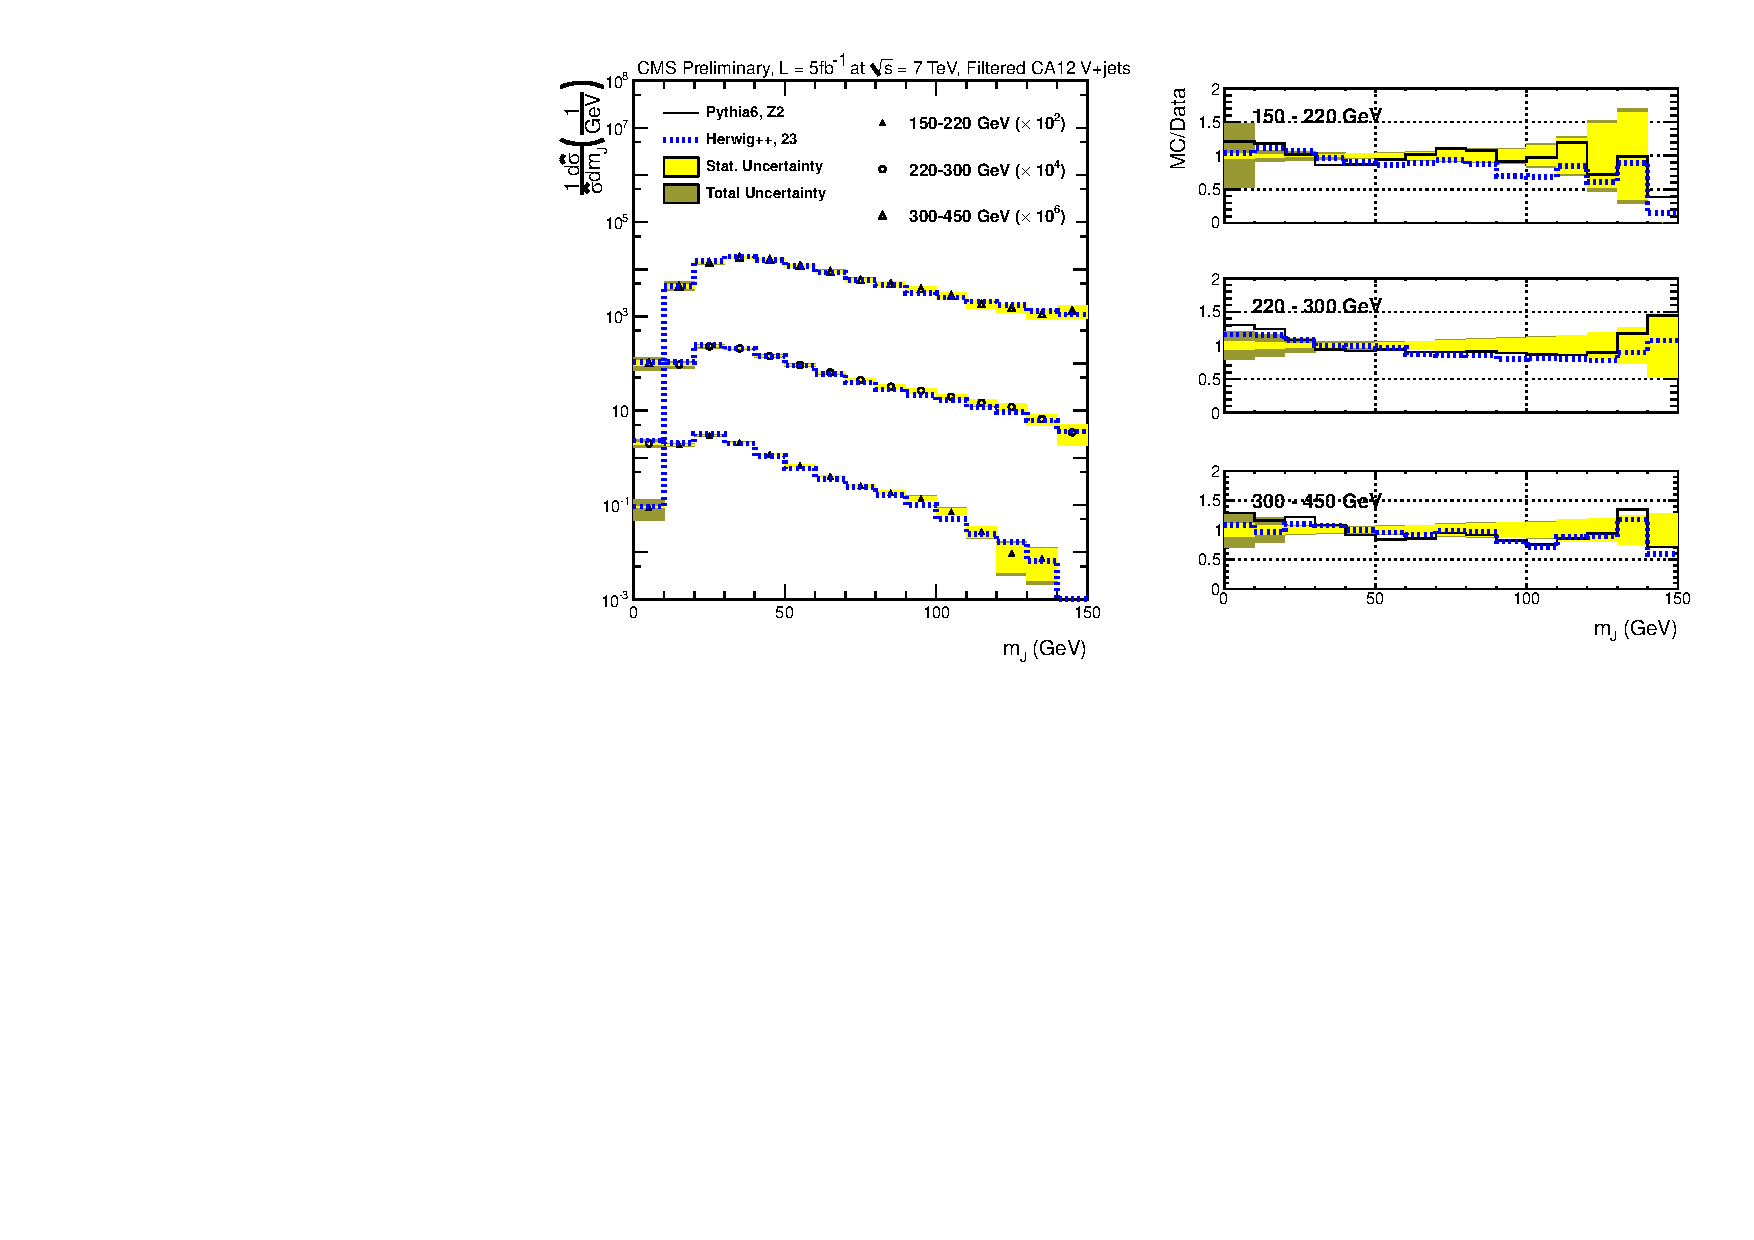
\includegraphics[width=0.99\textwidth]{figs/Wln/jetmassunf_ca12ft_log.pdf}
\caption{Unfolded CA 1.2 filtered jet mass distribution for W$(\ell\nu)$+ jet events. The data (black points) are compared to the MC expectations from Madgraph (solid red) and herwigpp (solid blue).}
\label{figs:prunedWmnInt2}
\end{figure}

\clearpage






